\documentclass[12pt]{article}
\usepackage[latin2]{inputenc}
\usepackage{t1enc}
\usepackage{amsmath}
\usepackage[magyar]{babel}
\usepackage{graphics}

\usepackage{fullpage}

\usepackage{float} %H-hoz


\title{Biztonságkritikus robotrepül\H{o}gép földi állomás\\ Specifikáció, összehasonlítás}
\author{Böjti Paszkál\\BH0R0N}
\begin{document}
\maketitle
%\tableofcontents

\section{Megoldások}
Számos megoldás született a földi állomás GUI\footnote{Graphics User Interface, grafikus megjelenítés}-jának kialakítására. Els\H{o}dleges követelmény, hogy az operátor mindig a legfontosabb információkat láthassa, ehhez szoftverergonómiailag kell megtervezni a m\H{u}szerek, adatok elrendezését.
Az alábbiakban összehasonlításra kerülnek a megjelenítési felületek.

\subsection{MIT GCS}
\cite{bib:mit}Els\H{o}dleges megfontolás az volt, hogy a m\H{u}szereket az értékeket linerisan jelenítsék-e meg, mivel az avionikában ez a kérdés már felmerült, így a valós m\H{u}szerek alapján a lineárisat választották. Másodlagos kérdés a m\H{u}szerek formája, itt megvalósítható lenne a csupán digitális értékek kiírása, de szintén a repülésb\H{o}l merítve a kör alakú egységeket választottak

\begin{figure}[H]
	\centering
	\resizebox{10cm}{!}{
		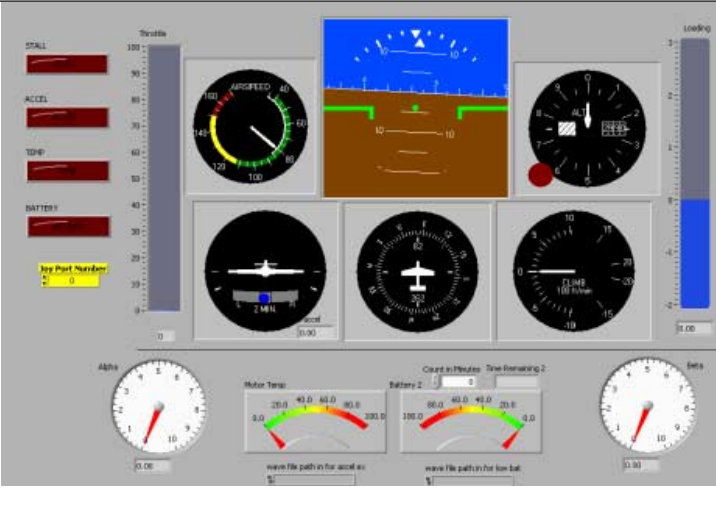
\includegraphics{mit.png}}
	\caption{Alap összeállítás}
	\label{fig:mit}
\end{figure}

\subsection{Rodan}
\cite{bib:rodan}Földi, légi, vízi jármüveket is támogat, TCP/IP-n keresztül kommunikál, így videó átküldésére is van sávszélesség. SIL\footnote{Software In the Loop} és HIL\footnote{Hardware In the Loop} támogatás.

A GUI itt már összetettebb, a kamera képe foglalja el a képerny\H{o} nagyobbik részét, mellette egy térképen láthatjuk a járm\H{u} eddigi útvonalát. Egyetlen vizuális m\H{u}szer a m\H{u}horizont, a többi érték csak számadattal van jelezve.

\begin{figure}[H]
	\centering
	\resizebox{10cm}{!}{
		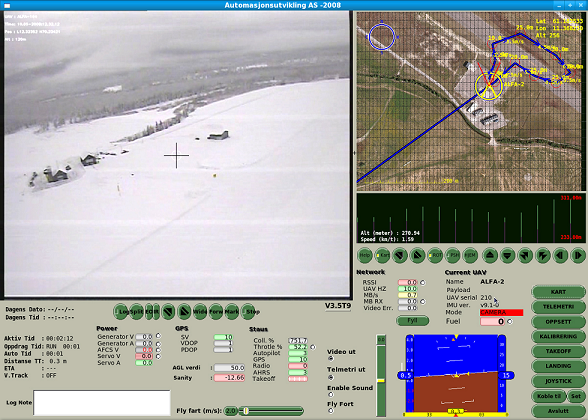
\includegraphics{rodan.png}}
	\caption{Rodan}
	\label{fig:rodan}
\end{figure}

\subsection{HappyKillmore}
\cite{bib:hk} Ez a GUI az ArduPlane nev\H{u} nyílt forráskódú, háziépítés\H{u} UAV-hoz készült.
Itt is a térkép nézet dominál, oldalt mozgathatjuk számunkra megfelel\H{o} elrendezésbe a m\H{u}szereket.
Több különböz\H{o} oldal közül választhatunk, ha pl. a bejöv\H{o} adatokra vagyunk kiváncsiak vagy a soros port port számát szeretnénk beállítani. Lehet\H{o}ségünk van exportálni is az adatokat.


\begin{figure}[!h]
	\centering
	\resizebox{10cm}{!}{
		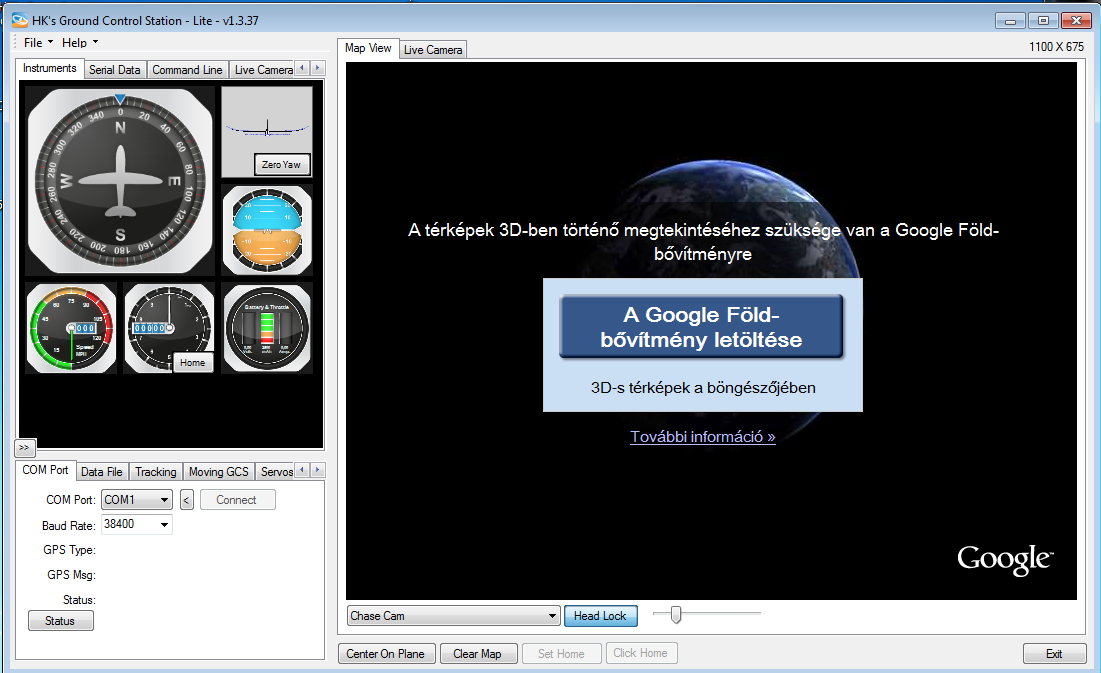
\includegraphics{hk.png}}
		\caption{HK}
	\label{fig:hk}
\end{figure}


\subsection{Arducopter}
Az el\H{o}z\H{o}höz hasonlóan ez is az ArduCopterhez készült. Itt lehet\H{o}ségünk van térképen el\H{o}re kijelölni, milyen útvonalat járjon be felszállás után.


\begin{figure}[H]
	\centering
	\resizebox{10cm}{!}{
		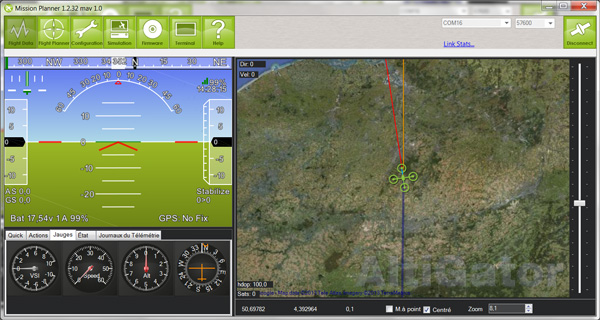
\includegraphics{ardu.png}}
	\caption{Arducopter}
	\label{fig:hk}
\end{figure}


\subsection{Viking}
\cite{bib:viking} Itt egyértelm\H{u}en a térkép feletti pozicíón van a hangsúly, jobb oldalt néhány m\H{u}szer, illetve a fontosabb adatok számokkal


\begin{figure}[H]
	\centering
	\resizebox{10cm}{!}{
		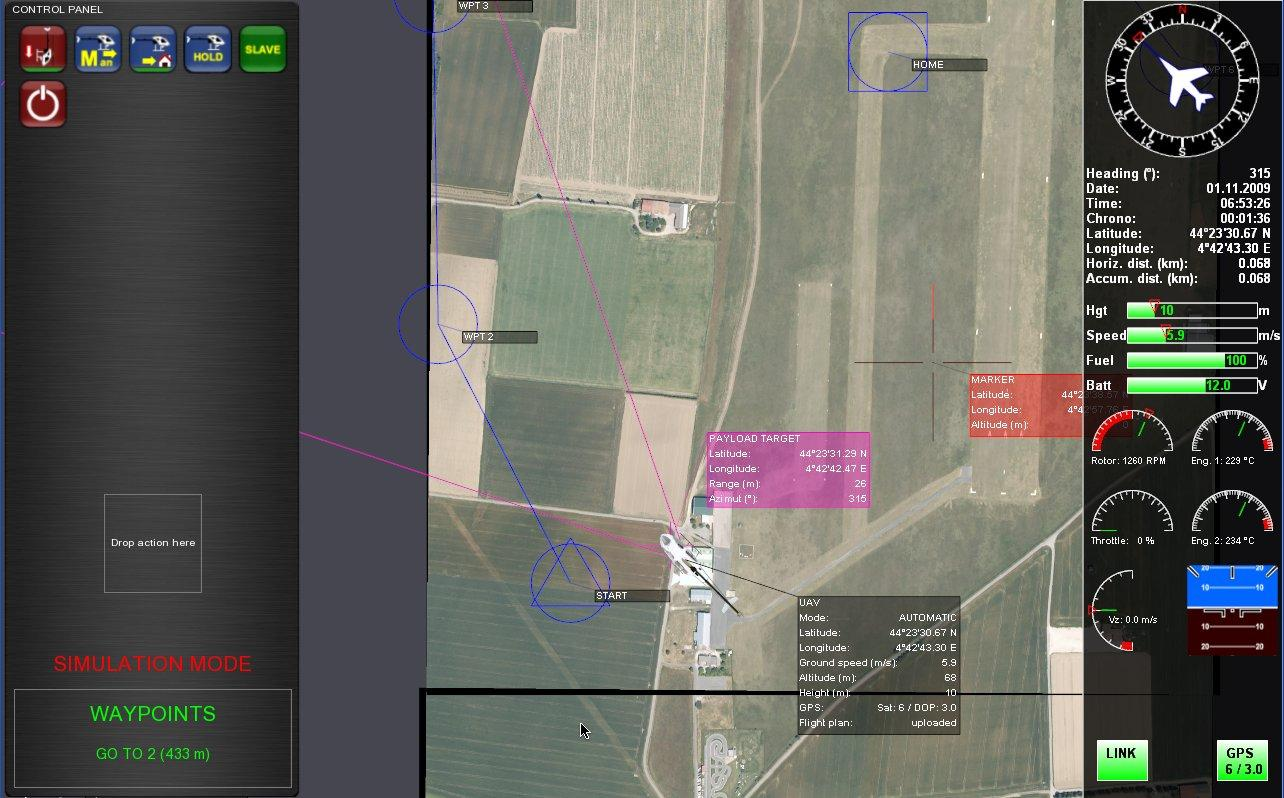
\includegraphics{viking.png}}
	\caption{Viking}
	\label{fig:viking}
\end{figure}

\section{.NET vs UNIX}
A .NET alapvet\H{o}en Microsoft technológia, de pl. a C\# könny\H{u} fejleszthet\H{o}sége miatt lehet\H{o}ségünk van .NET-ben írt alaklamazások UNIX rendszeren való futtatására is.
Erre szolgál segítségünkre a \cite{bib:mono}Mono több platformos rendszer, mely megvalósítja a .NET keretrendszert és a CLR\footnote{Common Language Runtime}-t, így ha úgy adódik, hogy a Ground Control állomás platformot vált, az eddig megírt program ,,portolható'' másik operációs rendszerre.

Tesztelhetjük is programjainkat, hogy kompatibilis-e a Monoval:
\begin{figure}[H]
	\centering
	\resizebox{10cm}{!}{
		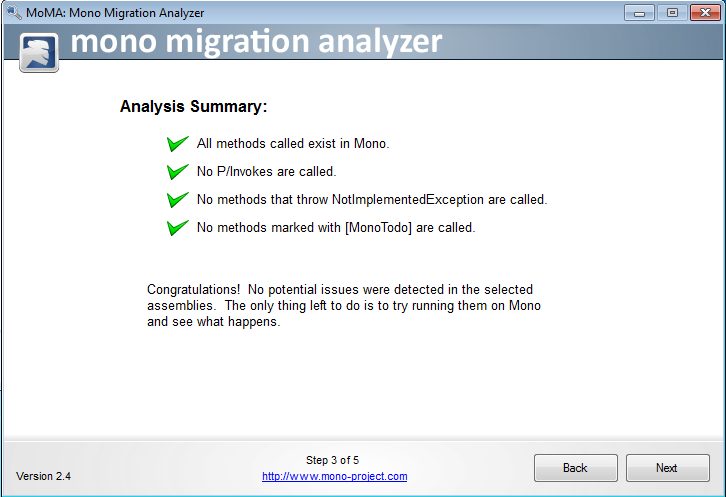
\includegraphics{mono1.png}}
	\caption{Mono}
	\label{fig:mono}
\end{figure}



\begin{thebibliography}{9}

\bibitem{bib:mit}
http://api.ning.com/files/ga5AVWy8xTu8cx9rHdzJ73Epc*dzb0uy*UPe0O8wFxogMF6WNRW8StK3x-xzkG2iBk16kNFpYTZe80NgM8kbXOiyxrEwUXIt/GroundControlStation.pdf, 2013.~március~19., 15:00

\bibitem{bib:rodan}
http://www.rodiangroup.com/uav-ground-control-station.html, 2013.~március~19., 15:00

\bibitem{bib:hk}
https://code.google.com/p/ardupilot-mega/wiki/HappyKillmore, 2013.~március~19., 16:00

\bibitem{bib:viking}

http://www.vikingaero.com/uav\_ground\_control\_station.html, 2013.~március~19., 16:00

\bibitem{bib:mono}
http://www.mono-project.com, 2013.~március~19., 17:00

\end{thebibliography}

\end{document}
